% TO DO: add book covers, discuss SVI and LDA example, maybe simple Dutch book but not so easy, use regularized regression as a red rope, with horseshoe as right subjective prior but also right frequentist prior provided EB is used to estimate the number of nonzero components.

\documentclass[10pt]{beamer}
\usetheme[height=0mm]{Rochester}
\usefonttheme[onlylarge]{structurebold}
\setbeamerfont*{frametitle}{size=\normalsize,series=\bfseries}
\setbeamertemplate{navigation symbols}{}
\setbeamercovered{dynamic}
\setbeamertemplate{itemize item}[triangle]
\setbeamertemplate{itemize subitem}[triangle]
%\useoutertheme{infolines}

%  use Darmstadt if commenting the next line
\usepackage[footheight=1em]{beamerthemeboxes}
\usepackage[natbib=true,backend=biber,citestyle=authoryear]{biblatex}
\bibliography{stats,../bib/stats,../bib/learning}

\usepackage{amsmath,amssymb,amsthm,bbm}             % AMS Math
\usepackage[utf8]{inputenc}
\usepackage[english]{babel}
\usepackage{myAlgorithm}
\usepackage{xcolor}
\usepackage{graphicx}
\usepackage{subfigure}
\usepackage{hyperref}
\usepackage{mathtools}
\usepackage{mathrsfs}
\usepackage{wasysym}
\usepackage{tikz}
\usetikzlibrary{bayesnet}
\usetikzlibrary{arrows}
\usepackage{url}

% notation
\DeclareMathOperator*{\argmax}{arg\,max}
\DeclareMathOperator*{\argmin}{arg\,min}
\newcommand{\cA}{\mathcal{A}}
\newcommand{\cS}{\mathcal{S}}
\newcommand{\cF}{\mathcal{F}}
\newcommand{\cX}{\mathcal{X}}
\newcommand{\cY}{\mathcal{Y}}
\newcommand{\cZ}{\mathcal{Z}}
\newcommand{\cN}{\mathcal{N}}
\newcommand{\cO}{\mathcal{O}}
\renewcommand{\leq}{\leqslant}
\renewcommand{\geq}{\geqslant}
\renewcommand{\phi}{\varphi}
\renewcommand{\epsilon}{\varepsilon}
\renewcommand{\d}{ {\rm d}}
\renewcommand{\emptyset}{\varnothing}

\newcommand\un[1]{\textcolor{magenta}{#1}}
\newcommand\unn[1]{\textcolor{blue}{#1}}
\newcommand\unnn[1]{\textcolor{red}{#1}}
\newcommand\unnnn[1]{\textcolor{orange}{#1}}

\def\cX{\mathcal{X}}
\def\cY{\mathcal{Y}}
\def\cZ{\mathcal{Z}}
\def\cS{\mathcal{S}}
\def\cR{\mathcal{R}}
\def\cA{\mathcal{A}}

\def\by{\mathbf{y}}

% indicator
\newcommand\IND[1]{\mathbbm{1}_{\{#1\}}}

\def\cfdemo{\url{https://chi-feng.github.io/mcmc-demo/}}

\def\tpi{\widetilde{\pi}}
\def\cN{\mathcal{N}}
\renewcommand\d{\mathrm{d}}
\def\e{\mathrm{e}}

\usecolortheme[named=bleu]{structure}

\title[Bayesian ML: what, why, and how?]{Bayesian ML: what, why, and how?}
\subtitle{Part 2: why would you want to use it?}
%\subtitle{\url{http://github.com/rbardenet/bml-course}}
\author[Rémi Bardenet (CNRS \& Univ. Lille)] % (optional, for multiple authors)
{Rémi Bardenet}
\institute[] % (optional)
{
  CNRS \& CRIStAL, Univ. Lille, France\\
  \url{http://rbardenet.github.io}\\
\vspace{1cm}

\includegraphics[width=0.15\textwidth]{Logos/logo_CNRS.pdf}
\qquad \includegraphics[width=0.35\textwidth]{Logos/logo_CRISTAL}
\qquad
\includegraphics[width=0.15\textwidth]{Logos/logo_ERC}
\qquad 
\includegraphics[width=0.13\textwidth]{Logos/logo_funded_by_ANR}
}
\date{}

\begin{document}
\begin{frame}
\maketitle
\end{frame}

\begin{frame}
\frametitle{Outline}
\tableofcontents
\end{frame}

\begin{frame}{Recap: posterior expected utility}
  \begin{block}{The subjective expected utility principle}
  \begin{enumerate}
  \item \un{Choose} $\cS, \cZ, \cA$ and a loss function $L(a,s)$,
  \item \un{Choose} a distribution $p$ over $\cS$,
  \item Take the the corresponding \un{Bayes action}
  \begin{equation}
  a^\star \in \argmin_{a\in\mathcal{A}} \mathbb{E}_{s\sim p} L(a,s).
  \label{e:seu}
  \end{equation}
  \end{enumerate}
  \end{block}
  \vfill

  \begin{block}{Corollary: minimize the posterior expected loss}
  If we partition $s=(s_{o}, s_{\text{u}})$, then
  $$ a^\star \in \argmin_{a\in\mathcal{A}} \mathbb{E}_{s_{o}} \mathbb{E}_{s_{\text{u}}\vert s_{o}} L(a,s).$$
  Equivalently to \eqref{e:seu}, given $s_o$, we choose
  $$
  a^\star = \delta(s_o) = \argmin_{a\in\mathcal{A}} \un{\mathbb{E}_{s_{\text{u}}\vert s_{o}} L(a,s)}.$$
  \end{block}
\end{frame}

\section{Because you abide by the likelihood principle}
\begin{frame}
\frametitle{The likelihood principle \citep{BeWo88}}
\begin{block}{The ``formal" LP}
  Consider two statistical experiments
  $$
  E_i=(X_i,\un{\theta}, \{p_i(\cdot\vert\vartheta), \vartheta\in\Theta\}), \quad i=1,2.
  $$
  Assume that for some realizations $x_1$ and $x_2$,
  $$
  p_1(x_1\vert\cdot) \propto p_2(x_2\vert \cdot).
  $$
  If $\text{Ev}(E,x)$ denotes the ``evidence on $\theta$ arising from $E$ and $x$", then
  $$
  \text{Ev}(E_1,x_1) = \text{Ev}(E_2,x_2).
  $$
\end{block}

\begin{exampleblock}{Corollary}
$\text{Ev}(E,x)$ can depend on $x$ solely through $p(x\vert\cdot)$.
\end{exampleblock}
\end{frame}

\begin{frame}
\frametitle{An example: model-based classification}
\end{frame}

\begin{frame}{Standard Bayes satisfies the LP}
\begin{itemize}
  \item Take $p_i(s_i) = p_i(x_i,\theta) = p_i(x_i\vert\theta)\un{p(\theta)} = \un{Z} p_i(\theta\vert x_i).$
  \item Then for $a:\cS\rightarrow\cZ$,
  $$ \int L(a,s_1) \frac{p_1(x_1\vert\theta)p(\theta)}{\un{Z}} \d\theta \propto \int L(a,s_2) \frac{p_2(x_2\vert\theta)p(\theta)}{\un{Z}} \d\theta, $$
  so that Bayes actions coincide: $a^\star = \delta_1(x_1) = \delta_2(x_2)$.
  \item However, full expected utilities are different in general:
  \begin{align*}
    \int L(a,s_1) p_1(x_1\vert\theta)p(\theta) \unn{\d x_1}\d\theta
    &\neq \int L(a,s_2) p_2(x_2\vert\theta)p(\theta) \unn{\d x_2}\d\theta.
  \end{align*}
\end{itemize}
\end{frame}

\begin{frame}
\frametitle{Pros and cons of the LP}
\begin{itemize}
  \item The LP is compelling to many \citep{BeWo88}, but it has its downsides.
  \item Being Bayesian is only one way to abide by the LP.
  \item I am personally uncomfortable with the stopping rule principle, probably because my frequentist intuition is still too strong.
  \item It is hard to make fully formal: is $\text{Ev}(E,x)$ even meaningful? See answer by LeCam to \citep{BeWo88}.
  \item It assumes we want to specify a likelihood, this prevents model-free Bayesianism.
  \item It separates the roles of the likelihood and the prior. For LP-abiding Bayesians, \un{the prior is not allowed to depend on data}.
\end{itemize}
\end{frame}

% ###############################################
\section{Because you place coherence above all things: subjective Bayes}
% ###############################################
\begin{frame}
  \frametitle{The subjectivistic viewpoint}
  \begin{itemize}
    \item Top requirement is \un{internal coherence} of decisions.
    \item Various attempts at proving that, internally, coherent decision-makers minimize some expected utility; see \citep{PaIn09}.
    \begin{figure}
      \centering
      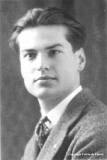
\includegraphics[width=\threefig]{\figdir/deFinetti.jpg}
      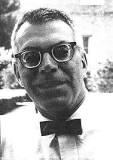
\includegraphics[width=\threefig]{\figdir/savage.jpg}
      \caption{Bruno de Finetti (1906--1985) and L. ``Jimmie" Savage (1917--1971)}
    \end{figure}
  \end{itemize}
\end{frame}

\begin{frame}{Savage's axioms 1/2}
\begin{itemize}
\item Start with the triple $(\cS,\cZ,\cA\subset \cF(\cS, \cZ))$ as in \cite{Wal50}.
\item Savage's idea is to list what we expect from a binary relation $\prec$ on $\cA\times \cA$ describing a decision maker's preferences.
\end{itemize}
\blank
\blank
\end{frame}

\begin{frame}{Savage's axioms 2/2}
\end{frame}

\begin{frame}{De Finetti's theorem (Hewitt-Savage form)}
  \begin{block}{Theorem: exchangeable $\leftrightarrow$ conditionally i.i.d.; see \citep[Theorem 1.49]{Sch95}}
    Let $X_1,X_2,\dots$ be a sequence of exchangeable random variables on $\cX$, i.e.
    $$
    X_1,\dots,X_n \sim X_{\pi(1)},\dots, X_{\pi(n)}, \forall n, \forall \pi\in\frak S_n.
    $$
    Then there exists a probability distribution $\mu$ \un{on the set of probability measures $\mathcal P(\cX)$ on $\cX$} such that
    $$
    \mathbb P (X_1\in A_1, \dots, X_n\in A_n) = \int Q(A_1)\dots Q(A_n)\d\mu(Q).
    $$
    Furthermore, if $Q\sim\mu$,
    $$
    Q(A) = \lim_{n\rightarrow\infty} \frac 1n\sum_{i=1}^n 1_A(X_i).
    $$
  \end{block}
  To a subjectivist, Savage's theorem says you should use SEU, and representation theorems like de Finetti's constrain your choice of $p$.
\end{frame}

\begin{frame}{De Finetti's theorem and LDA}
\end{frame}

\begin{frame}{De Finetti's theorem and Bayesian nonparametrics}
\end{frame}

\begin{frame}{Bonus: The Dirichlet process through de Finetti's theorem}

\begin{block}{The Blackwell-McQueen urn scheme (aka the CRP)}
  Start with an urn containing a single black ball with weight $\alpha$. Repeat: draw a ball from the urn with probability $\propto$ its weight. Then,
  \begin{itemize}
    \item If the ball is black, return it to the urn along with another ball of weight 1, with a new color sampled from some base measure $H$.
    \item If the ball is colored, return it to the urn along with another ball of weight 1 of the same color.
  \end{itemize}
  Denote by $X_1,\dots$ the color of the ball added.
\end{block}
\vfill
\begin{itemize}
  \item Exercise: show that $X_1,X_2,...$ are exchangeable.
  \item The corresponding prior $\mu$ on $\mathcal{P}(\cX)$ is the Dirichlet process with concentration $\alpha$ and base measure $H$.
\end{itemize}
\end{frame}

\begin{frame}{Pros and cons of the subjectivist viewpoint}
\end{frame}

% % ###############################################
% \subsection{Logic/positivist Bayesians}
% % ###############################################
% \begin{frame}
%   \frametitle{The logical justification}
%   \begin{itemize}
%     \item Top requirement is to find a version of propositional logic that allows taking into account uncertainty.
%     \item Also favourizes interpreting \un{probability distributions as beliefs}, but aims for objective priors.
%     \begin{figure}
%       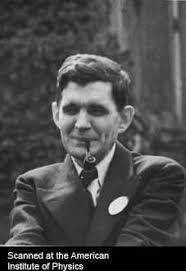
\includegraphics[width=\threefig]{\figdir/cox.jpg}
%       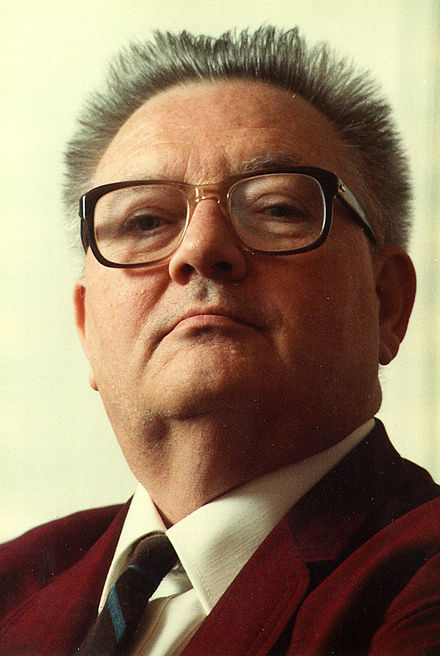
\includegraphics[width=\threefig]{\figdir/jaynes.jpg}
%       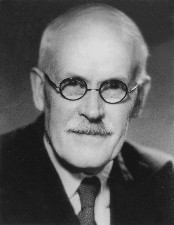
\includegraphics[width=\threefig]{\figdir/jeffreys.jpg}
%       \caption{Richart T. Cox (1898--1991), Edwin T. Jaynes (1917--1971), and Harold Jeffreys (1891--1989)}
%     \end{figure}
%   \end{itemize}
% \end{frame}

% ###############################################
\section{Because you like coherence and consensus: objective Bayes}
\begin{frame}{Objective Bayes}
\begin{itemize}
\item A historical objection to Bayes is the need to choose a prior.
\item By ``objective", we mean that the prior is chosen by some external rule, and that this rule is relatively consensual.
\item Take for instance, Jeffreys's ``noninformative" priors.
\blank
\end{itemize}
\end{frame}
% ###############################################

\section{Because you want to be a good (Waldian) frequentist}

\begin{frame}{Complete class theorems state that there is a good prior (but which one?)}

\begin{block}{A complete class theorem for estimation \citep{Ber85}}
Under topological and Euclidean assumptions, if further \begin{itemize}
\item $L(\theta,\cdot)$ is continuous,
\item $\theta\mapsto \int L(\theta,\hat\theta)p(y_{1:n} \vert x_{1:n}, \theta)\d y_{1:n}$ is continuous for any $\hat\theta$,
\end{itemize}
then \un{for any estimator $\tilde\theta$} there exists a prior and a corresponding Bayes estimator
$$
\hat\theta_{\text{Bayes}} \in \argmin_{\hat\theta} \mathbb{E}_{\theta\vert x_{1:n},y_{1:n}} L(\theta,\hat\theta)
$$
such that
$$ \forall \theta, \quad \mathbb E_{y_{1:n}\vert x_{1:n},\theta} L(\theta,\hat\theta_{\text{Bayes}}) < E_{y_{1:n}\vert x_{1:n},\theta} L(\theta,\tilde\theta).$$
\end{block}
\begin{alertblock}{Bayesian estimators thus have good frequentist properties}
But finding the ``right" prior can be difficult. Frequentists typically use Bayesian derivations with particular (often data-dependent) priors; see e.g. empirical Bayes procedures \citep{Efr10}.
\end{alertblock}
\end{frame}

\begin{frame}{Sparse Bayesian regression}
\end{frame}

\subsection{PAC-Bayesian learning}
\begin{frame}{PAC-Bayesian learning}
\begin{block}{PAC bounds; see e.g. \citep{ShBe14}}
Let $(x_{1:n},y_{1:n})\sim \mathbb{P}^{\otimes n}$, and independently $(x,y)\sim \mathbb{P}$, we want an algorithm $g(\cdot; x_{1:n}, y_{1:n})\in\mathcal G$ such that if $n\geq n(\delta,\epsilon)$,
$$
\unn{\mathbb{P}^{\otimes n}}\left[\mathbb{E}_{(x,y)\sim \mathbb P} L(a_g,s) \leq \epsilon\right] \geq 1-\delta.
$$
\end{block}
\begin{block}{McAllester's bound for 0-1 loss (Chapter 31 of the above book)}
For any two distributions $P,Q$ on $\mathcal G$, with $\unn{\mathbb{P}^{\otimes n}}$-probability $1-\delta$,
$$
\mathbb E_{g\sim Q} \un{\mathbb{P} (g(x)\neq y)} \leq \mathbb{E}_{g\sim Q} \unnnn{\frac1n\sum_{i=1}^n 1_{g(x_i)\neq y_i}} + \sqrt{\frac{\text{KL}(Q,P) + \log(n/\delta)}{2(n-1)}}.
$$
\end{block}

This suggests taking the ``posterior" $Q$ to be in
$$
\argmin \mathbb{E}_{g\sim Q} \unnnn{\frac1n\sum_{i=1}^n 1_{g(x_i)\neq y_i}} + \sqrt{\frac{\text{KL}(Q,P) + \log(n/\delta)}{2(n-1)}}.
$$
\end{frame}

\section{Most modern Bayesians are hybrid Bayesians}
\begin{frame}
  \frametitle{One possible hybrid view, e.g. \citep{Rob07}}
  \begin{itemize}
    \item The starting point is Wald's decision setting, adding integration with respect to a prior.
    \item It is simple, widely applicable, has good frequentist properties.
    \item It satisfies the \un{likelihood principle} when priors do not depend on data.
    \item It is tempting to interpret it as follows: beliefs are
    \begin{itemize}
      \item represented by probabilities,
      \item updated using Bayes' rule,
      \item integrated when making decisions.
    \end{itemize}
    \item It is easy to communicate your uncertainty
    \begin{itemize}
      \item Simply give your posterior.
      \item When making a decision, make sure that the priors of everyone involved would yield the same decision.
      \item Alternately, perform a \un{prior sensitivity analysis}.
    \end{itemize}
  \end{itemize}
\end{frame}

\section{Discussion}
\begin{frame}{What kind of Bayesian are you?}
\begin{itemize}
\item I've only scratched the surface. See e.g. \citep{May18}.
\item Posterior expected utility is conceptually simple and unifying. Beyond that, \un{many intepretations get partial philosophical support}.
\item The role of the likelihood, the prior, your update mechanism, etc. \un{depend} on the intepretation that you choose.
\item[\frownie] \un{Many people do not care}.
\item Hybrid views have become common \citep{Rob07,GCSDVR13}. This arguably makes the role of priors fuzzy.
\item In ML, the development of \un{Bayesian nonparametrics is reviving the subjectivist view}, while objective approaches like \un{PAC-Bayes are also increasingly popular}.
\item A great door to subjective Bayes is \citep{PaIn09}.
\end{itemize}
\end{frame}
  


% From linear regression to GPs
% Example regression
% Bayesian optimization
% Applications to hyperparameter tuning

%\includegraphics[width=.9\textwidth]{salsify}

\section*{References}
\setbeamertemplate{bibliography item}[text]%,
\begin{frame}[allowframebreaks]
\frametitle{References}
\small
\printbibliography
\normalsize
\end{frame}
\end{document}
